%% Available options for the mengthesis documentclass:

%% Option `11pt':
%%   Use an 11pt font (10pt by default).

%% Option `12pt':
%%   Use an 12pt font (10pt by default).

%% Option `draft':
%%   Puts `overfull' boxes at the end of lines that are too long.

%% Option `leftblank':
%%   If using the `twoside' option, marks extra blank pages with ``THIS PAGE
%%   INTENTIONALLY LEFT BLANK''.

%% Option `mitcopyright':
%%   Gives the thesis copyright to MIT instead of the author.

%% Option `singlespace':
%%   Single-spaces the document, for drafts (double-spaced by default).

%% Option `twoside':
%%   Prints double-sided, inserting extra blank pages as necessary.

\documentclass[twoside,leftblank,mitcopyright]{mengthesis}

% Very basic packages you'll likely need for graphics, symbols, PDF hyperlinking, etc
\usepackage{xcolor, graphicx, gensymb, amssymb, amsmath, textcomp, hyperref}

% Helps manage floats and prevent them from going into the next section
% ex: use \FloatBarrier to prevent any floats from going that point in the doc 
\usepackage{placeins}

% Tables with more column flexibility
\usepackage{tabularx}

% Customize formatting of captions
\usepackage[hang, small, bf, margin=20pt, tableposition=top]{caption}

% Better done ToCs
\usepackage{tocloft}

% Allows areas of text to be excluded from processing, ex: \begin{xcomment} blah \end{xcomment}
\usepackage{xcomment}

% Creates ordinal number suffixes/formatting like 1st, 2nd, etc. ex: \engordnumber{2} 
\usepackage{engord}
% command for "0th"
\newcommand{\zeroth}{0$^{\rm th}$}


% Define centered expanding width column
\newcolumntype{C}{>{\centering\arraybackslash}X}

% Used for subfigures
\usepackage{subfig}
\captionsetup[subfigure]{format=hang, margin=5pt}

% Use EPS files in PDFLatex
\usepackage{epstopdf}

% Define colors for the todo list
%\usepackage{atveryend} % prereq for todonotes
% Get \marginpar to work properly on odd/even pages
%\usepackage{mparhack}
%\setlength{\marginparwidth}{2cm} % hack to get todonotes to play with MEng template
%\definecolor{todonotesbg}{rgb}{1, 0.678431373, 0.631372549}
%\usepackage[colorinlistoftodos, color=todonotesbg,bordercolor=red,textsize=footnotesize]{todonotes}
%\newcommand{\todo}{}  %If you need to disable todo temporarily

% Prettifies Tables - ex: \toprule, \bottomrule, \midrule
\usepackage{booktabs}

% Easily use acronyms - ex: \acronym{SN}{supernova}, \ac{SN},  
\usepackage[printonlyused,withpage]{acronym}

% Allow rotated tables, figures, etc
\usepackage{rotating}

% Side captions, ex: \begin{SCfigure}
\usepackage{sidecap}

% Embed PDF pages in document, ex: \includepdf[pages=1-4]{Myfile.pdf}
\usepackage{pdfpages}

% Setup the Hypertext PDF linking
\hypersetup{
    bookmarks=true,         % show bookmarks bar?
    unicode=false,          % non-Latin characters in Acrobat’s bookmarks
    pdftoolbar=true,        % show Acrobat’s toolbar?
    pdfmenubar=true,        % show Acrobat’s menu?
    pdffitwindow=false,     % window fit to page when opened
    pdfstartview={FitH},    % fits the width of the page to the window
    pdftitle=My Spiffy Thesis,    % title
    pdfauthor=My Awesome Name,     % author
%   pdfsubject={Subject},   % subject of the document
%    pdfcreator={Creator},   % creator of the document
%    pdfproducer={Producer}, % producer of the document
%    pdfkeywords={keywords}, % list of keywords
    pdfnewwindow=true,      % links in new window
    colorlinks=true,       % false: boxed links; true: colored links
    linkcolor=black,          % color of internal links
    citecolor=blue,        % color of links to bibliography
    filecolor=magenta,      % color of file links
    urlcolor=cyan           % color of external links
}

% Compacted itemize- less white space inbetween items
\usepackage{enumitem}  % compact enumerates and itemizes, ex: \begin{enumerate*}...
\newenvironment{packed_itemize}{
\begin{itemize}[label=\textbullet, nolistsep, leftmargin=10pt,
            before*={\mbox{}\vspace{-\baselineskip}}]
  \setlength{\itemsep}{2pt}
  \setlength{\parskip}{0pt}
  \setlength{\topsep}{0pt}
  \setlength{\partopsep}{0pt}
  \setlength{\parsep}{0pt}
}{\end{itemize}}
\newenvironment{subpacked_itemize}{
\begin{itemize}[label=\textbullet, nolistsep, leftmargin=10pt]
  \setlength{\itemsep}{2pt}
  \setlength{\parskip}{0pt}
  \setlength{\topsep}{0pt}
  \setlength{\partopsep}{0pt}
  \setlength{\parsep}{0pt}
}{\end{itemize}}

% Remove citations from ToC, ToF, etc..., Ex: none, works automatically
\usepackage{notoccite}

% Force LaTex to not change spacing between paragraphs
\setlength{\parskip}{8pt}

% For floats, Ex: \float[H]...
\usepackage{float}

% For floating figures with text wrap. Ex: \begin{wrapfigure}{r}{0.5\textwidth}
\usepackage{wrapfig}

% Force compacted white space between chapter and section titles
\usepackage[compact,rigidchapters]{titlesec}

\begin{document}

%=============================== CONFIGURATION ===============================%

%% Specify your thesis title.

\title{My Spiffy Thesis}

%% Specify your full name.

\author{My Awesome Name}

%% If you wish to list your previous degrees on the cover page, use the
%% previous degrees command:
%%       \prevdegrees{A.A., Harvard University (1985)}
%% You can use the \\ command to list multiple previous degrees
%%       \prevdegrees{B.S., University of California (1978) \\
%%                    S.M., Massachusetts Institute of Technology (1981)}

\prevdegrees{S.B., Massachusetts Institute of Technology (2006)}

%% Specify the month and year you'll be graduating, and the exact date to put
%% on the thesis.
\degreemonth{February}
\degreeyear{2010}
\thesisdate{February 10, 2010}

%% By default, the thesis will be copyrighted to you.  If you need to copyright
%% the thesis to MIT, just specify the `mitcopyright' documentclass option.  If
%% for some reason you want to exactly specify the copyright notice text, you
%% can use the \copyrightnotice command.

%\copyrightnotice{Copyleft 2009 John E. Doe.  All rights reversed.}

%% Use the \supervisor command to specify the name and title of your thesis
%% supervisor.  If there is more than one supervisor, use the \supervisor
%% and/or \cosupervisor command once for each.

% For your advisor's proper title: http://eecsfacweb.mit.edu/gallery.html
\supervisor{My Advisor's Name}
           {My Advisor's Title}


%============================= DOCUMENT PREAMBLE =============================%

%% Create a title page, as specified by the Course-VI M.Eng. Thesis Guide.
\pdfbookmark[0]{Title Page}{title} % Sets a PDF bookmark for the title page
\maketitle

%% Acknowledgements

%% Create the TOC; feel free to add lists of figures/tables after this.

%% Begin "Page Left Blank" hack for forcing ToC/LoF/etc to start on odd numbered page- you may need to remove this!
\clearpage
\hbox{}\par\vfill\centerline%
   {THIS PAGE INTENTIONALLY LEFT BLANK}%
   \vfill\newpage
   \thispagestyle{plain}
\clearpage
%% End "Page Left Blank" hack

\pdfbookmark[0]{Contents}{contents} % Sets a PDF bookmark for the contents page
\tableofcontents

%% Begin "Page Left Blank" hack for forcing ToC/LoF/etc to start on odd numbered page- you may need to remove this!
\clearpage
\hbox{}\par\vfill\centerline%
   {THIS PAGE INTENTIONALLY LEFT BLANK}%
   \vfill\newpage
   \thispagestyle{plain}
\clearpage
%% End "Page Left Blank" hack

%% Create the List of Figures
\listoffigures

%% Create the List of Tables
\clearpage % You may need to remove this!
\listoftables

%% Begin "Page Left Blank" hack for forcing ToC/LoF/etc to start on odd numbered page- you may need to remove this!
\clearpage
\hbox{}\par\vfill\centerline%
   {THIS PAGE INTENTIONALLY LEFT BLANK}%
   \vfill\newpage
   \thispagestyle{plain}
\clearpage
%% End "Page Left Blank" hack

%================================= CHAPTERS ==================================%
% abstract.tex
%% Create a abstract page, as specified by the Course-VI M.Eng. Thesis Guide.
%% Careful to use the special "abstractpage" environment here, rather than the
%% usual "abstract" environment.
\begin{abstractpage}
\pdfbookmark[0]{Abstract}{abstract} % Sets a PDF bookmark for the abstract

The proliferation of dynamic program analysis tools has done much to ease the
burden of developing complex software.  However, creating such tools remains a
challenge.  Dynamic binary instrumentation frameworks such as DyanamoRIO and
Pin provide support for such tools by taking responsibility for application
transparency and machine code manipulation.  However, tool writers must still
make a tough choice when writing instrumentation: should they inject custom
inline assembly into the application code, or should they use the framework
facilities for inserting callbacks into regular C code?  Custom assembly can be
more performant and more flexible, but it forces the tool to take some
responsibility for maintaining application transparency.  Callbacks into C, or
``clean calls,'' allow the tool writer to ignore the details of maintaining
transparency.  Generally speaking, a clean call entails switching to a safe
stack, saving all registers, materializing the arguments, and jumping to the
callback.

This thesis presents a suite of optimizations for DynamoRIO that improve the
performance of ``na\"ive tools,'' or tools which rely primarily on clean calls
for instrumentation.  Most importantly, we present a novel {\em partial
inlining} optimization for instrumentation routines with conditional analysis.
For simpler instrumentation routines, we present a novel {\em call coalescing}
optimization that batches calls into fewer context switches.  In addition to
these two novel techniques, we provide a suite of machine code optimizations
designed to leverage the opportunities created by the aforementioned techniques.

With this additional functionality built on DynamoRIO, we have shown
improvements of up to 54.8x for a na\"ive instruction counting tool as well as a
3.7x performance improvement for a memory alignment checking tool on average for
many of the benchmarks from the SPEC 2006 CPU benchmark suite.

\end{abstractpage}

\chapter*{Acknowledgements}

This thesis was made possible with the help of many individuals.  First and
foremost, Saman Amarasinghe, my advisor, has provided me with the guidance
needed to complete the project, for which I am grateful.  I also want to thank
him for making 6.035, the MIT undergraduate compilers course, as rigorous and
practical as it was.  Derek Bruening also deserves much credit for being the
driving force behind DynamoRIO.  Working closely on DynamoRIO, I have learned
more and more about the transparency and performance challenges that it faces
and how they have been overcome.  Qin Zhao, another contributor to DynamoRIO,
has helped me a great deal through conversation about the implementation details
of the system.  Qin is also responsible for the initial inlining prototype,
which I have been working steadily to improve.  I have learned something new
after every one of our conversations.

On a more personal note, I thank my parents for everything they have given me.
To my father, I have always enjoyed our conversations, technical and otherwise.
To my mother, I am ultimately thankful for the time you have spent encouraging
me to achieve.

%People:

%Saman, for advising and 6.035 and 6.172

%Qin, for DR advice

%Derek, for DR advice

%Marek and Jason, feedback at group meetings

%Erica

%Parents?


%% Nomenclature- for acronyms
\chapter*{Nomenclature}
\begin{acronym}[]

% Example acronyms
\acro{2D}{Two Dimensional}
\acro{3D}{Three Dimensional}
\acro{ch}{channel}
\acroplural{ch}[ch]{channels}
\acro{km}{kilometer}
\acro{kms}[km/s]{kilometers/second}
\acroplural{kms}[km/s]{kilometers/second}

\end{acronym}
\acresetall % Reset the acronym definitions

\chapter{Introduction}

\section{Research Objectives}

Dynamic program analysis tools built with dynamic binary instrumentation have
proven indispensable for developing largs applications in C and C++.
Valgrind's\cite{valgrind} memory debugger in particular has been instrumental in
tracking down uses of uninitialized memory and memory leaks.  Race detectors
such as Helgrind\cite{helgrind} and Thread Sanitizer\cite{tsan} have made
programming with shared memory feasible.  Cache simulators and branch prediction
simulators such as Cachegrind\cite{valgrind_workloads} provide a way to optimize
cache usage in a given program.

These are just the most commonly used types of instrumentation tools.  However,
researchers in academia and industry are building new general-purpose as well as
application-specific tools.  For example, a research group at MIT recently
created Jolt\cite{jolt}, a tool for detecting and escaping from infinite loops
with Pin\cite{pin}.  During the work for this thesis, I developed a tool for to
identify which routines in an application perform unaligned memory accesses,
which can hurt performance.

For the last several years, Pin has been the framework of choice for
implementing new custom program analysis tools.  Pin's success in this area is
explained in the creators' PLDI paper, which focuses on Pin's facilities for
abstracting away architectural details from the instrumentation tool.  A Pin
tool works by inserting calls to instrumentation routines, which record
information about the program execution.  For example, it is common for a Pin
tool to instrument every memory access to call to a function with information
about that memory access.  Furthermore, if the instrumentation routine is small
enough, Pin can decode the routine and inline it into the application code
stream.

On the other hand, DynamoRIO\cite{bruening_phd} has a larger and more general
interface.  Instead of only inserting calls to plain C or C++ routines, a tool
has the power to insert custom machine code into the application code.  For
example, PiPa\cite{pipa} is a cache simulator that inserts custom assembly to
fill a buffer with application memory access information.  Another thread
consumes the data to simulate the cache using pipeline parallelism.  DrMemory,
a memory debugger built with DynamoRIO, generates memory accesses that will
fault if the application uses uninitialized data.  While faulting is expensive,
it happens rarely, and in the common case of the access succeeding is faster
than a normal conditional branch.

Being able to insert custom machine code is powerful and can support highly
efficient tools, but it is a daunting task for a researcher or a beginner
learning the framework.  To help ameliorate the burden, DynamoRIO also has
facilities for inserting ``clean calls,'' which are similar to Pin's
instrumentation routines.  However, DynamoRIO cannot inline clean calls, and is
generally not suited to pervasive instrumentation using clean calls.

The goal of this thesis is to make it possible to build performant program
anlysis tools with DynamoRIO without burdening the tool writer.  Throughout
this thesis, we follow the efforts of a tool author attempting to implement
three tools: an instruction counting tool, a memory alignment tool, and a
memory access trace tool.  To support the author of these tools, we make the
following contributions:

\begin{packed_itemize}
\item An {\em inlining} optimization for instrumentation routines.
\item The first {\em partial inlining} optimization for instrumentation
routines with conditional analysis.
\item The first {\em call coalescing} optimization for instrumentation
routines.
\item A suite of x86 machine code optimizations leveraging the opportunities
created by inlining.
\end{packed_itemize}

Partial inlining is a well-understood compiler optimization that attempts to
inline the commonly executed code without inlining an entire function, which
would cause code bloat.  In our case, not all tool code is possible to inline
into the application code stream, so partial inlining can help by making
inlining possible at all.  As far as we know, this is the first use of this
technique to dynamic instrumentation tools.

For tools built with pervasive clean calls, the main cost for such a tool is
usually the context switching between the application and DynamoRIO.  The idea
behind call coalescing is that we should make multiple calls after one context
switch so that we need to make fewer context switches over all.

Finally, we found that applying the above techniques was not enough, and that
we needed to build a larger suite of general machine code optimizations to
finish cleaning up the inlined code.  For example, in our memory alignment
tool, the size used for the alignment check is passed as a parameter, and it is
always the same at each call site.  If we inline without folding this constant
into the alignment check, we are clobbering extra registers and issuing extra
instructions.

%{\em To Saman: Would you rather have me delete the thesis overview section
%below and move the few paragraphs up here giving more detail about partial
%inlining?  I feel like the overview is redundant with the table of contents.}

Using the above techniques, we have been able to dramatically improve
performance for an instruction counting tool by 54.8 times and a memory
alignment tool by almost 4 times.

\section{Thesis Overview}

In Chapter \ref{sec:background} we discuss the motivation for using a dynamic
binary instrumentation framework such as DynamoRIO, Pin, or Valgrind in the
first place.  In particular, we outline all the benefits they provide and
challenges they help overcome.  We also take a closer look at the execution
model of DynamoRIO because it has a great impact on the design of analysis
tools.

In Chapter \ref{sec:inlining} we start with a na\"ive implementation of
instruction count and walk through the stages of optimizations that we apply.
As we go through the stages, the instrumentation code is progressively
simplified until it starts to look like the version we would write using custom
machine code.

In Chapter \ref{sec:partial_inlining} we take a look at two more complex tools:
a memory alignment checker and a memory trace tool.  These tools have the common
property that the instrumentation has an early conditional check that results
either in a fast or a slow path being taken.  In the memory alignment tool, no
action needs to be taken if the memory access is aligned.  In the memory trace
tool, the trace buffer does not need to be flushed if it is not full.  We
describe how we go about inlining the fast paths while maintaining correctness
when the slowpath is taken.

In Chapter \ref{sec:system} we depart from our example-driven description of
the system to step back and look at the system hierarchy.

In Chapter \ref{sec:performance} we present the experimental performance results
we achieved on the SPEC2006 CPU integer benchmarks\cite{spec_cpu_2k6} for all
three of the tools examined in this thesis.

In Chapter \ref{sec:contributions} we look back on the contributions of this
thesis and suggest possible directions for future work.


\chapter{Background}
\label{sec:background}

% Background on design of DynamoRIO, all relevant considerations.

%%%%%%%%%%%%%%%%%%%%%%%%%%%%%%%%%%%%%%%%%%%%%%%%%%%%%%%%%%%%%%%%%%%%%%%%%%%%%%%%
\section{Dynamic Binary Instrumentation Frameworks}

In order to understand this thesis, it is important to understand what a dynamic
binary instrumentation (DBI) framework provides to a tool writer.

The primary job of a DBI framework is to interpret a native application as it
executes and provide an abstract representation of the program code that the
tool can analyze and instrument.  At first, it would seem easier to simply
disassmble the application in question and insert instrumentation code into it
statically.  However, for modern applications, this approach simply does not
work.  First, there are dynamically loaded libraries that the application may be
linked against.  Some of these are possible to identify, such as {\tt libc} or
others.  Some, however, may be dynamically loaded via other interfaces such as
{\tt dlopen} on Linux and {\tt LoadLibrary} on Windows.  These are not possible
to predict statically, and a static instrumentation tool will not be able to
observe and instrument these instructions.  Hence, a {\em dynamic} binary
instrumentation framework is needed to run alongside the application and
intercept every instruction that the application would have executed were it to
run natively.  Using dynamic instrumentation instead of static instrumentation,
an analysis tool can observe and manipulate {\em all} instructions executed by
the application instead of just some.

Furthermore, a dynamic framework maintains control even in the face of such
convoluted techniques as self-modifying code.  As techniques such as embedded
Just In Time (JIT) compilation become more prevalent, it becomes more important
to be able to observe such dynamically generated code.  A DBI framework is also
responsible for providing all of the native operating system interfaces to the
application just as if the application were running natively.  This can be a
daunting challenge, as the operating system interface is large, and an
application can register many points of entry with the operating system such as
signal handlers.  A good DBI framework, such as DynamoRIO, Pin, or Valgrind,
will intercept all of these requests and ensure that control is maintained and
the tool author is able to observe all instructions.

Finally, a DBI framework provides transparency of the framework and the tool to
the application.  When trying to analyze a program, it can be frustrating when
bugs disappear when run under the analysis tool.  If the tool and the framework
are completely transparent, then the application will not be able to tell that
it is running under the tool.  Furthermore, the tool will not affect the flow
of the application in any way.  For example, DynamoRIO provides a heap that is
fully isolated from the application, so memory allocations by the tool do not
disturb allocations by the application.  A separate heap also prevents
application bugs from overwriting DynamoRIO's data structures.  After heap data
structures, we also need to worry about the application's stack, for all of the
same reasons.  The application may have buffer overruns on the stack, or it
might not even have a stack.  Therefore, DynamoRIO maintains a separate stack.
Applications also occasionally use introspection to enumerate all the threads
in a process, query virtual memory protections, or walk the stack, for example.
DynamoRIO makes sure that all of these application introspection techniques
work as if they were running natively, so the tool author does not have to
worry about it.

For all of these reasons, it is highly desirable to build dynamic program
analysis tools with DBI frameworks.  The goal of this thesis is to make it
easier to use DBI frameworks to write analysis tools that perform well.  For
this thesis, we chose to start by modifying DynamoRIO, which we describe in the
following section.

%%%%%%%%%%%%%%%%%%%%%%%%%%%%%%%%%%%%%%%%%%%%%%%%%%%%%%%%%%%%%%%%%%%%%%%%%%%%%%%%
\section{DynamoRIO's Execution Model}

\begin{figure}
\begin{center}
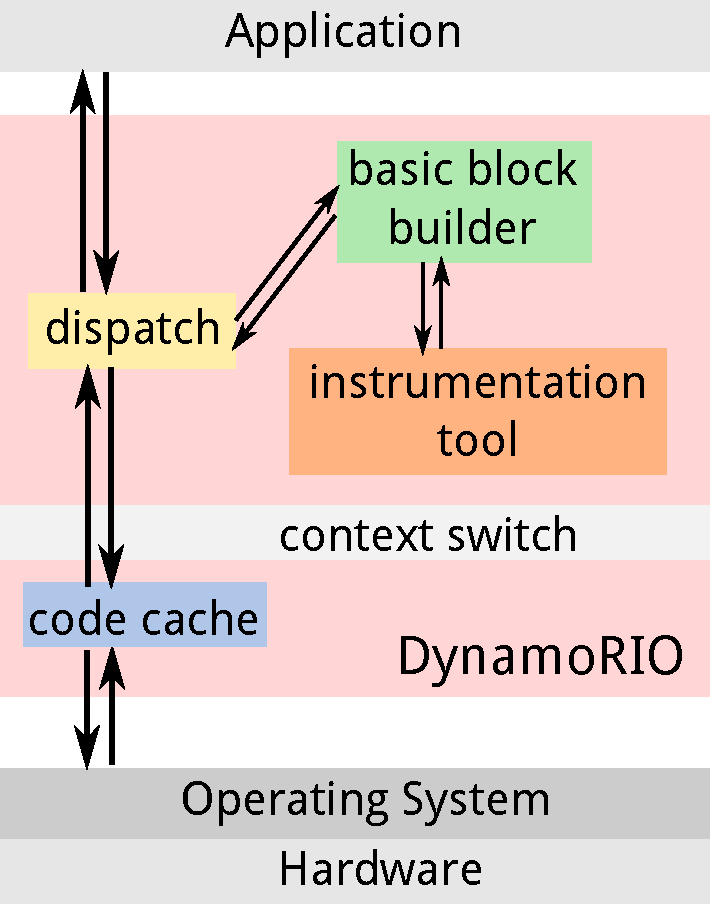
\includegraphics[width=3in]{tool-flow.pdf}
\caption{High-level diagram of DynamoRIO executing an application.}
\label{fig:tool-flow}
\end{center}
\end{figure}

In order to dynamically instrument an application, DynamoRIO performs ``process
virtualization.''  All application code is translated into the software code
cache, just as is done in VMWare's flagship virtualization
product.\cite{vmware_comparison}  Essentially, DynamoRIO injects itself between
the application and the operating system, as shown in Figure
\ref{fig:tool-flow}, instead of between the operating system and the hardware,
as VMWare does.  All control transfers between the application and the operating
system are caught and mediated by DynamoRIO so that it can maintain control.  To
run an application under DynamoRIO, the application is launched in such a way
that DynamoRIO is loaded and given control during process initialization.

When DynamoRIO takes control, it sets up its own execution context, separate
from that of the application.  DynamoRIO's context consists of a separate stack,
and a thread-local data structure describing its state.  The application context
consists of the original application stack along with all of the registers that
DynamoRIO may clobber while executing its own code.  Once DynamoRIO has switched
to its own stack, it determines what the next application program counter would
have been and begins the process of interpretation, entering the basic block
builder from Figure \ref{fig:tool-flow}.

For a previously unencountered target application PC, the builder decodes
instructions from the first instruction until the next control transfer.  Before
modifying the instructions to run in the code cache, DynamoRIO presents the
instructions to the tool for instrumentation, if a tool is loaded.  The tool
then has the opportunity to analyze the basic block and insert its own
instructions or clean calls.  Such instructions are marked as ``meta,'' meaning
they are not application instructions and should not be modified to maintain
control.  Inserting custom code into the application is the most efficient way
to perform analysis, but most na\"ive clients will stick to inserting clean
calls.  Clean calls require a full context switch across the gray border, and
significantly bloat code size, requiring extra memory and polluting the cache.

After instrumentation, DynamoRIO mangles the terminating control transfer
instruction to maintain control when the basic block exits.  Specifically,
control flow instructions are mangled so that they jump into DynamoRIO's central
dispatch mechanism which will figure out what to do next, which is represented
by the arrow leaving the code cache and entering the dispatch block in Figure
\ref{fig:tool-flow}.

Once DynamoRIO is done modifying the application instruction stream, the
instructions are encoded into a ``fragment'' in the code cache.  The code cache
is the memory space allocated by DynamoRIO for translated application code.
Finally, DynamoRIO switches back to the application context and starts executing
the new fragment.

When the basic block finishes execution, instead of transferring to the original
application target, it will re-enter the DynamoRIO VM with information about the
original target application program counter.  If the target application PC is
not in the code cache yet, DynamoRIO will then repeat the process of translation
for the next basic block.  After translation, it will return to the application
context and continue execution from the freshly translated fragment.

Bouncing back and forth between DynamoRIO's central dispatch and the code cache
is expensive, so DynamoRIO attempts to ``link'' basic blocks together.  If the
control transfer target is direct, the two basic blocks can be linked by
modifying the terminating control transfer instruction of the previous fragment
to directly target to the beginning of the next fragment.  As a result, when a
code path executes more than once, it will not have to leave the code cache to
look up the next fragment to execute.

Now that we have presented the motivations and challenges involved with dynamic
binary instrumentation, we demonstrate how simple inlining and our suite of
optimizations work together to optimize a na\"ive instruction counting tool.


\input{design}

\input{usability}

\input{results}

\input{conclusions}

%================================= APPENDIX ==================================%

\input{appendix}

%=============================== BIBLIOGRAPHY ================================%

% Force the PDF bookmarks to include the References
\clearpage
\phantomsection 

\renewcommand{\bibname}{References}  % Rename the bibliography to referances

\begin{singlespace}
\bibliographystyle{ieeetr} % Use the IEEE style- citations are numbered in order of appearance in the doc
\addcontentsline{toc}{chapter}{References} % Add to the table of contents
\bibliography{thesis}
\end{singlespace}

%=============================================================================%
\end{document}
